\section{Dwi Yulianingsih}
\subsection{Teori}
\subsubsection{Soal 1}
Device Manager dalam system operasi Windows, merupakan perluasan dari Microsoft Management Console. Device Manager akan menampilkan seluruh hardware yang bisa di-inisialisasi (dikenali) oleh system operasi Windows. Tampilannya ter-organisir sedemikian hingga yang akan memudahkan pengelolaan setiap hardware yang ada.
Fungsi-fungsi kegunaan Device Manager antara lain sebagai berikut :
\begin{itemize}
\item Menunjukkan status suatu hardware
\item Menunjukkan informasi detail suatu hardware
\item Mengelola driver hardware
\item Disable \& Enable hardware
\item Meng-identifikasi konflik antar hardware, dll.
\end{itemize}
Directory pada /dev berisi file device, baik device blok maupun device karakter. di dalamnya sekurangd-kurangnya  harus memiliki file biner MAKEDEV untuk membuat device ini secara manual.

\subsubsection{Soal 2}
\begin{itemize}
\item Hubungkan sistem minimun Arduino Uno ke komputer dengan kabel USB type B (kabel Printer).
\item Lalu pada bagian kanan didesktop PC anda, akan muncul popup “Installing device driver software” seperti pada gambar dibawah ini.
\item SIstem operasi Windows tidak menyediakan driver untuk Arduino Uno seperti yang terlihat pada gambar dibawah ini, lalu proses instalasinya harus dilakukan secara manual.
\item Buka Device Manager, caranya pada bagian Search Program and Files lalu ketikkan “device manager” (tanpa tanda petik), perhatikan gambar dibawah ini. Pada bagian Control Panel akan muncul Device Manager, klik untuk menjalankan.
\item Cari Unknown device pada bagian Other device, biasanya terdapat tanda seru berwarna kuning, itu disebabkan karena penginstallan tidak berjalan dengan sempurna.
\item Klik kanan pada “Unknown device” kemudian pilih Update Driver Software.
\item Pilih Browse my computer for driver software.
\item Arahkan lokasi folder ke folder ..arduino1.0.5 drivers. Pastikan checkbox lalu centang include subfolders. Klik Next untuk melanjutkan instalasi driver.
\item Kemudian lanjutkan dengan mengklik Install pada tampilan Windows Security.
\item Jika instalasi driver berhasil maka akan muncul Windows has successfully updated your driver software.
\item Perhatikan dan ingat nama COM Arduino Uno, karena nama COM ini yang akan digunakan untuk meng-upload program nantinya.
\end{itemize}

\subsubsection{Soal 3}
Hubungkan Port USB pada Arduino dengan Port USB komputer.
Buka Software Arduino pada Komputer.
Tuliaskan program berikut ini pada Arduino Sketch.

\subsubsection{Soal 4}
Modul ini merangkum akses untuk port serial. Ini menyediakan backends untuk Python yang berjalan di Windows, Linux, BSD (mungkin sistem yang mendukung POSIX), Jython dan IronPython (.NET dan Mono). Modul bernama "serial" secara otomatis memilih backend yang sesuai. Antarmuka berbasis kelas yang sama pada semua platform yang didukung.
Akses ke pengaturan port melalui properti Python. 
Dukungan untuk berbagai ukuran byte, bit stop, paritas dan kontrol aliran dengan RTS / CTS dan / atau Xon / Xoff.
Bekerja dengan atau tanpa menerima batas waktu.
File seperti API dengan "read" dan "write" ("readline" dll. Juga didukung).
File-file dalam paket ini adalah 100 persen Phyton murni.
Port diatur untuk transmisi biner. Tidak ada stripping byte NULL, terjemahan CR-LF dll. (Yang berkali-kali diaktifkan untuk POSIX.) Ini membuat modul ini bermanfaat secara universal.
Kompatibel dengan pustaka io (Python 2.6+).

\subsubsection{Soal 5}
Fungsi-fungsi yang dipakai dari library Pyserial, diantara :
\begin{itemize}
\item Serial – fungsi ini untuk membuka port serial
\item Write(data) – untuk menulis data lewat port serial
\item Readline() – untuk membaca string dari port serial
\item Read(size) – untuk membaca jumlah byte dari port serial
\item Close() – ini untuk menutup port serial 
\end{itemize}

\subsubsection{Soal 6}
Perualangan dalam bahasa pemrograman berfungsi menyuruh komputer melakukan sesuatu secara berulang-ulang. Terdapat dua jenis perualangan dalam bahasa pemrograman python, yaitu perulangan dengan for dan while. Perulangan for disebut counted loop (perulangan yang terhitung), sementara perulangan while disebut uncounted loop (perulangan yang tak terhitung). Perbedaannya adalah perulangan for biasanya digunakan untuk mengulangi kode yang sudah diketahui banyak perulangannya. Sementara while untuk perulangan yang memiliki syarat dan tidak tentu berapa banyak perulangannya. Perulangan diperlukan agar dapat membaca data secara berulang kali sehingga data yang muncul lebih dari satu.  Sedangkan apabila tidak memakai perulangan maka data akan terbaca satu kali saja.

\subsubsection{Soal 7}
Berikut merupakan contoh penggunaan fungsi yang menggunakan pyserial
\lstinputlisting[firstline=8, lastline=15]{src/5/1174009/T1174009.py}

\subsubsection{Bukti bebas plagiarisme}
\begin{figure}[H]
\centering
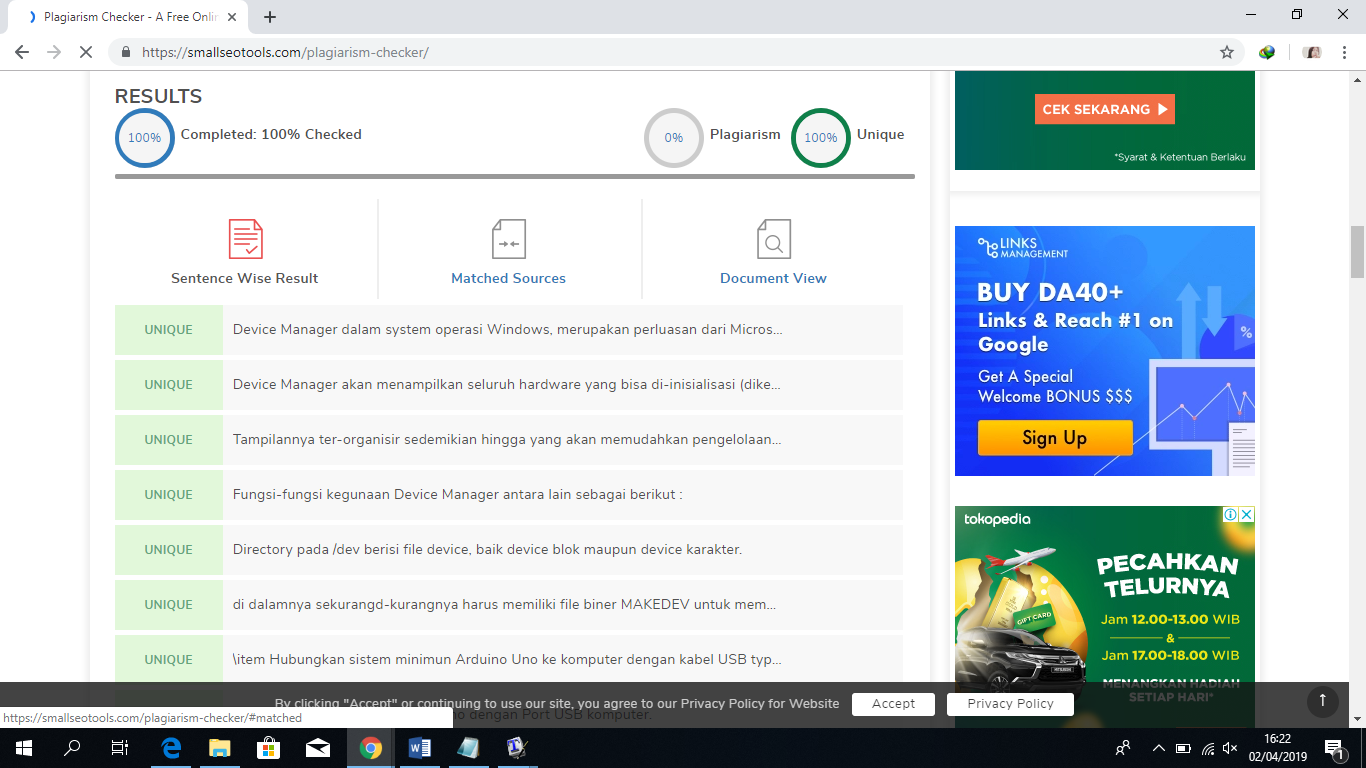
\includegraphics[width=10cm]{figures/5/1174009/plagi.png}
\caption{SS Bebas Plagiarisme}
\label{dwiyul}
\end{figure}

\subsection{Praktek}
\begin{enumerate}
\item Soal 1
\lstinputlisting[firstline=8, lastline=14]{src/5/1174009/1174009_realtime.py}

\item Soal 2
\lstinputlisting[firstline=8, lastline=15]{src/5/1174009/1174009_save.py}

\item Soal 3
\lstinputlisting[firstline=16, lastline=29]{src/5/1174009/1174009_realtime.py}

\item Soal 4
\lstinputlisting[firstline=8, lastline=16]{src/5/1174009/1174009_csv.py}

\end{enumerate}

\subsubsection{Penanganan Error}
cara untuk menangani eror yang dapat dilakukan adalah sebagai berikut:
\lstinputlisting[firstline=8, lastline=17]{src/5/1174009/1174009_eror.py}